\documentclass[12pt]{article}

\usepackage{graphicx}
\usepackage[caption=false]{subfig}
\usepackage[margin=2.5cm, a4paper]{geometry}
\usepackage{dcolumn}
\usepackage{bm}
\usepackage{amsmath}
\usepackage{hyperref}
\usepackage{xcolor}
\usepackage{braket}  % Bra-ket notation
\usepackage{float}
\usepackage{tikz}

\setlength\parindent{0pt}

\title{Supporting Informations: Computational Approach to Ultrafast Hydrogen Bonding in Water and Ice}
\author{Author(s)}
\date{\today}

\begin{document}

\maketitle

\clearpage

\section*{Wigner Sampling of Hydrogen-Bonded O--H\,$\cdots$\,O Coordinates}

The initial conditions for the nonequilibrium simulations were generated
by sampling the phase-space distribution associated with hydrogen-bonded
O--H\,$\cdots$\,O configurations using a Wigner formalism.


\begin{figure}
	\begin{center}
		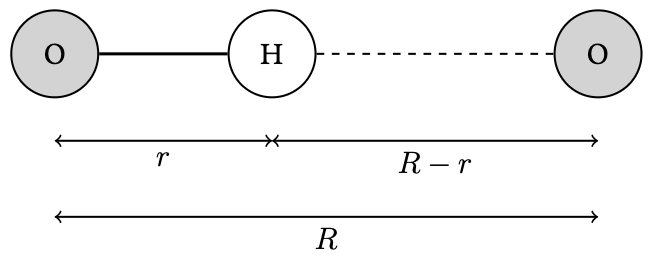
\includegraphics[width=0.6\textwidth]{si_figures/LS-schema.png}
	\end{center}
	\caption{}\label{fig:}
\end{figure}



\subsection*{Effective one-dimensional hydrogen-bond coordinate}

Instead of treating the O--H bond as an isolated intramolecular degree of
freedom, we considered an effective one-dimensional coordinate describing
the motion of the hydrogen atom along the O--H\,$\cdots$\,O direction. This
coordinate captures both the covalent O--H stretching and its coupling to
the hydrogen-bond interaction with a neighboring oxygen atom.\\

The corresponding potential energy surface was modeled using the
Lippincott-Schroeder parametrization of the form:

\[
	V(r) = V_{\mathrm{O-H}}(r) + V_{\mathrm{H\cdots O}}(r),
\]

With

\[
	\begin{aligned}
		 & V_{\mathrm{O-H}}(r) = D_{OH} \left( 1 - \exp\left[
		-\frac{n(r-r_0)^2}{2r}\right]\right)                  \\
		 & V_{\mathrm{O\cdots H}}(r) = - D^* \exp\left[
			-\frac{n^*(R - r - r_0^*)^2}{2(R -r)}\right]
	\end{aligned}
\]

Where:

\begin{itemize}
	\item[$r$] represent the Hydrogen position in respect to the covalent bonded
	      oxygen;
	\item[$D_{OH}$] represent the $O-H$ bond dissociation energy;
	\item[$n$] is the covalent stiffness parameter;
	\item[$r_0$] is the covalent bond equilibrium distance;
	\item[$D^*$] represent the hydrogen bond dissociation energy and is obtained
	      as $D_{OH} / g^*$;
	\item[$n^*$] represent the hydrogen bond stiffness and is obtained
	      as $n \cdot g^*$;
	\item[$r_0^*$] is the
	\item[$R$]

\end{itemize}

Following ANDO, the modified Lippincott--Schroeder potential was
parameterized using $g = 1.45$ and $r_0^* = 0.95\,r_0$. Here, $g$
controls the relative curvature and depth of the hydrogen-bond term
through $n^* = g\,n$ and $D^* = D_{\mathrm{OH}}/g$, whereas $r_0^*$
sets the effective equilibrium position of the acceptor-side
interaction. Together, these parameters introduce the physically
required asymmetry of the O--H$\cdots$O potential, avoiding an
artificially symmetric proton-sharing double well.


\subsection*{Quantum vibrational states}

The vibrational eigenstates associated with this effective coordinate were
obtained by solving the one-dimensional Schrödinger equation

\[
	\left[
		- \frac{\hbar^2}{2\mu} \frac{d^2}{dr^2} + V(r)
		\right] \psi_n(r) = E_n \psi_n(r),
\]

where $\mu$ is an effective reduced mass dominated by the hydrogen atom.

This construction implicitly incorporates the anharmonicity of both the
covalent bond and the hydrogen-bond interaction.

\subsection*{Wigner phase-space distribution}

For each selected vibrational eigenstate $\psi_n(r)$, the corresponding
Wigner distribution was computed numerically as

\[
	W_n(r,p) =
	\frac{1}{\pi \hbar}
	\int_{-\infty}^{\infty}
	\psi_n(r+y)\,\psi_n(r-y)\,
	e^{2 i p y / \hbar} \, dy.
\]

The integral was evaluated on a finite grid using numerical quadrature,
with interpolation of the wavefunction values to ensure numerical stability.

\subsection*{Sampling and mapping to atomic coordinates}

Phase-space points $(r,p)$ were sampled using an acceptance--rejection
scheme based on the absolute value of the Wigner distribution.

Each sampled configuration was mapped onto atomic coordinates by modifying
the position of the hydrogen atom along the O--H\,$\cdots$\,O axis. The
sampled momentum $p$ was converted into a velocity component along the same
axis and assigned to the hydrogen atom, with corresponding adjustments
ensuring conservation of momentum within the molecular unit.

This procedure selectively initializes fluctuations along the
hydrogen-bond coordinate while preserving the underlying molecular
structure.

\subsection*{Remarks}

The present approach extends standard Wigner sampling of intramolecular
vibrations by explicitly including the hydrogen-bond degree of freedom,
thereby capturing the coupled nature of O--H stretching and intermolecular
interactions. While the subsequent dynamics is propagated classically, this
initialization provides a quasi-classical representation of quantum
fluctuations in hydrogen-bonded systems.
\end{document}
